\chapter{Управление по выходу с заданной степенью устойчивости}
\label{ch:chap2}
\section{Условие задачи}

Рассмотреть систему:
$$
  \begin{cases}
    \dot{x} = Ax + Bu \\
    y = Cx
  \end{cases}
$$ и выполнить следующие шаги:

\begin{itemize}
    \item  Найти собственные числа матрицы $A$ и определить наблюдаемость каждого из них. 
    Сделать вывод об наблюдаемости и обнаруживаемости системы.
    \item Определить, любой ли желаемой степени устойчивости вы можете добиться от
данной системы при помощи регулятора вида $u = Kx$. Объяснить, почему, и, если не любой, то определить максимальную возможную.
    \item  Определить, любой ли желаемой степени сходимости вы можете добиться от наблюдателя 
    полной размерности для данной системы. Объяснить, почему, и, если не любой, то определить максимальную возможную.
  \item Построить схему моделирования системы замкнутой регулятором $u = Kx$ с наблюдателем $\dot{\hat{x}} = A\hat{x} + Bu + L(C\hat{x} - y)$
  \item Задаться не менее чем парой значений $\alpha > 0$, все из которых могли бы быть
  использованы в качестве желаемой степени устойчивости для регулятора и желаемой 
  степени сходимости для наблюдателя. Если существуют ограничения на достижимые 
  степени устойчивости или сходимости, то одна из выбранных $\alpha$ должна
  быть максимально возможной, а другие достижимыми. Постарайтесь взять достаточно 
  отличающиеся значения $\alpha$.
\item Используя выбранные значения $\alpha$, составить не менее чем 
3 набора значений желаемой степени устойчивости $\alpha_K$ и желаемой степени сходимости $\alpha_L$, 
среди которых должны быть случаи равенства, и неравенства в обе стороны.

Для каждого из выбранных наборов:

\begin{itemize}
  \item Найти соответствующую матрицу регулятора $K$, обеспечивающую желаемую $\alpha_K$. 
  Отклонения фактических собственных чисел спектра замкнутой системы от желаемой
  степени устойчивости должны быть \textbf{минимизированы}.
  \item Определить собственные числа матриц замкнутых систем $(A+BK)$ и сравнить 
  с желаемой степенью устойчивости в подтверждение корректности синтеза регулятора.
  \item Найти соответствующую матрицу наблюдателя $L$, обеспечивающую желаемую степень сходимости $\alpha_L$. 
  Отклонения фактических собственных чисел спектра наблюдателя от желаемой степени сходимости должны быть \textbf{минимизированы}.
  \item Определить собственные числа матриц замкнутых систем $(A+LC)$ и сравнить с желаемой степенью устойчивости в подтверждение корректности синтеза наблюдателя.
  \item Выполнить моделирование с начальными условиями системы 
  $x(0) = \begin{bmatrix} 1&1&1&1 \end{bmatrix}^T$ и наблюдателя $\hat{x}(0)=\begin{bmatrix}0 & 0& 0 &0\end{bmatrix}^T $.
  Построить  сравнительные графики $x(t)$ и $\hat{x}(t)$, график управления $u(t)$ и ошибки наблюдателя
   $e(t) = x(t) - \hat{x}(t)$.
  
\end{itemize}
\item Сравнить полученные результаты для различных наборов $\alpha_K$ и $\alpha_L$ 
сделать выводы о взаимном влиянии степени устойчивости регулятора и степени 
сходимости наблюдателя при управлении по выходу.
\end{itemize}
    
\newpage
\section{Решение задачи}

Параметры для объекта:
$$
  A = \begin{bmatrix}
    5  &  -7   & -5  &   1 \\
   -7   &  5  &  -1   &  5 \\
   -5  &  -1  &   5   &  7 \\
    1  &   5  &   7   &  5

  \end{bmatrix} \tab
  B = \begin{bmatrix}
    5\\7\\1\\9
  \end{bmatrix} \tab
  C = \begin{bmatrix}
    0 & 0 & 2 & 2\\
    1 & 1 & -1 & -1
  \end{bmatrix}
$$

\subsection{Исследование наблюдаемости и управляемости системы}
Найдём собственные числа матрицы $A$:
$$
    \sigma(A) = \{-8, 4, 8, 16\}
$$
Обратимся к исследованию в моей прошлой работе - система будет полностью наблюдаема и управляема, 
а значит все собственные числа этой системы будут тоже наблюдаемы и управляемы.

В таком случае мы сможем добиться любой степени устойчивости/сходимости, посколько мы вправе сдвигать все собственные числа для синтеза
регулятора/наблюдателя, а значит
степень устойчивости будет зависеть от нашего выбора $\alpha$. 

Построим аналогичную схему с предыдущей работы:

\begin{figure}[ht]
  \centering
  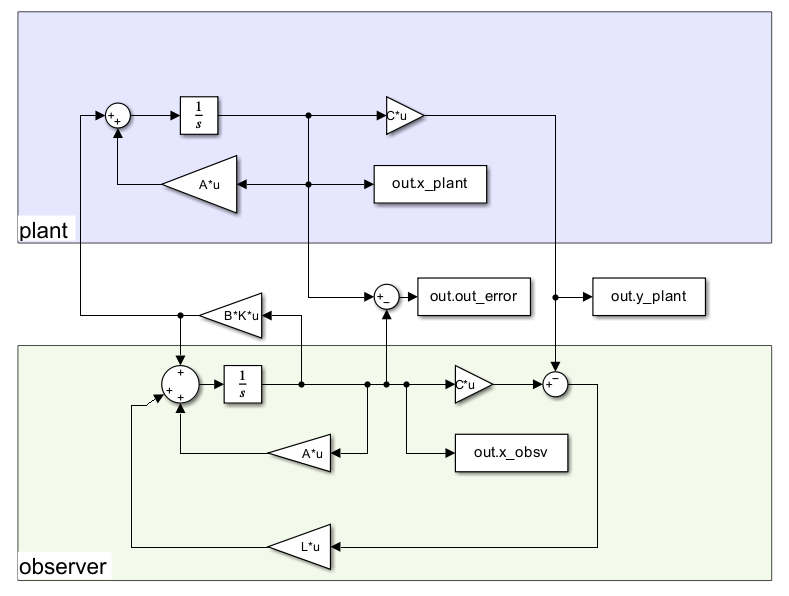
\includegraphics[width=0.6\textwidth]{model_observer_controller.png}
  \caption{Модель с модальным регулятором и наблюдателем}
\end{figure}

\newpage
\subsection{Желаемая степень сходимости и устойчивости}
При нашей конфигурации системы мы можем добиться любой степени сходимости и устойчивости, 
поскольку система неустойчива изначально, но полностью управляема/наблюдаема, 
поэтому регулятор может вольно перенести собственные числа в соответствии с выбранным $\alpha$
Выберем пару значений коэффициентов сходимости $\alpha$:
$$
  \alpha_{1,2} = \{ 3, 11 \} 
$$
Составим наборы значений параметров $\alpha$ и проведём исследование.
\subsection{Наблюдатель и регулятор равны}
$$
  \alpha_K = \alpha_L = 3
$$
Найдём матрицу регулятора $K$ \textbf{методом матричных неравенств Ляпунова}, минимазацию отклонения фактических собственных чисел замкнутой системы от заданного параметра добьёмся минимазицией, 
которую обеспечат два дополнительных матричных неравенства отдельной задачей по минимизации управления:

Для такой степени устойчивости синтезируем регулятор при помощи \textbf{матричного уравнения Риккати}:
$$
\begin{cases}
  PA^T + AP + 2\alpha P + Y^TB^T \preceq 0, \tab P \succ 0 \\
  K = YP^{-1} \\
  \begin{bmatrix}
    P & x_0 \\
    x_0^T & 1
  \end{bmatrix} \succ 0,  \tab \rightarrow \tab \mu = 26 \\
  \begin{bmatrix}
    P & Y^T \\
    Y &\mu^2I
  \end{bmatrix} \succ 0, \tab \rightarrow \tab 
  K_1 = \begin{bmatrix}
   17.32 & -19.84 & 3.84 &  1.28
  \end{bmatrix}
\end{cases}
$$
Регулятор даст следующий спектр, у нас сейчас $\alpha_K = 3$:
$$
  \sigma(A+BK_1) = \{-4.83 \pm 23.74i, -4.84, -7.97 \}
$$
Судя по спектру, регулятор синтезирован корректно. 

Теперь синтезируем наблюдателя при помощи \textbf{матричного уравнения Риккати}, 
уравнения и неравенства будут выглядеть лишь чуть по-другому:
$$
\begin{cases}
  A^T Q + QA + 2\alpha Q + C^T Y^T + YC \preceq 0 \\
  L = Q^{-1}Y \\
  \begin{bmatrix}
    Q & e_0 \\
    e_0^T & I
  \end{bmatrix} \succ 0,  \tab \rightarrow \tab \mu = 15 \\
  \begin{bmatrix}
    Q & Y \\
    Y^T &\mu^2I
  \end{bmatrix} \succ 0, \tab \rightarrow \tab 
  L_1 = \begin{bmatrix}
    18.43 &  -7.06 \\
   -21.39 &  0.08 \\
    -4.43 &  7.19 \\
    -7.39 &  0.20 \\
  \end{bmatrix}
\end{cases}
$$
Где $e_0 = x_0 - \hat{x}_0$ - отклонение 'начальных' условий. Наблюдатель даст следующий спектр, у нас сейчас $\alpha_L = 3$:
$$
  \sigma(A+L_1 C) = \{-3.18 \pm 14.68i, -8, -3.1 \}
$$
Судя по спектру, наблюдатель синтезирован корректно, так как он не превышеает заданной $\alpha$.

\newpage
\begin{figure}[ht]
  \centering
  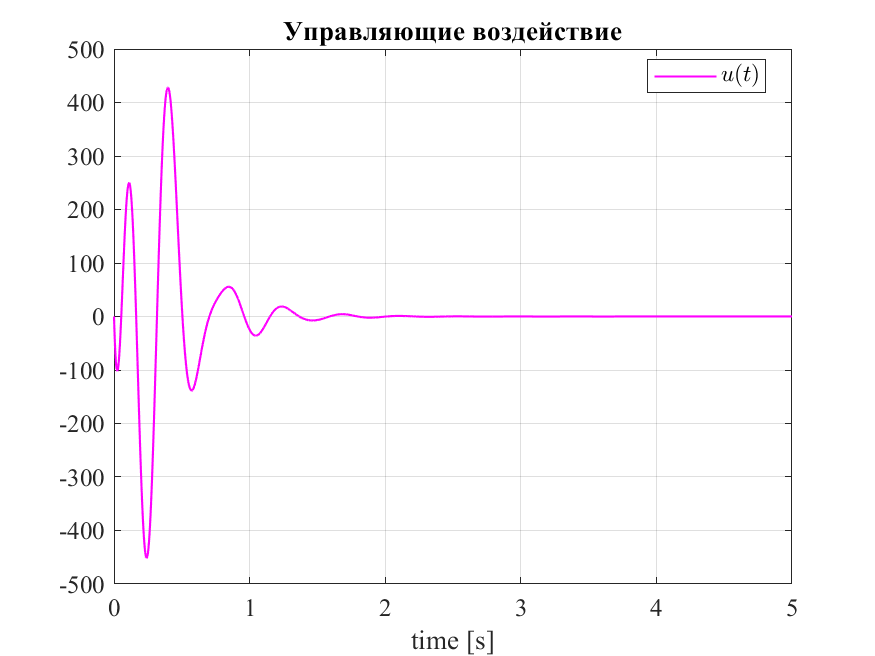
\includegraphics[width=0.8\textwidth]{obsv_u1.png}
  \caption{Сигнал управления и регулятор}
\end{figure}
\begin{figure}[ht]
  \centering
  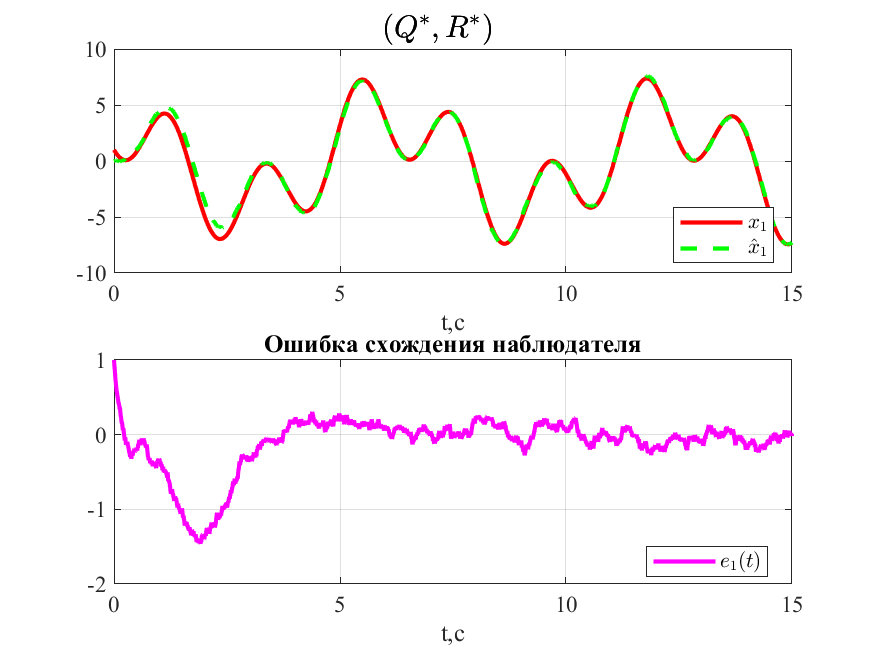
\includegraphics[width=0.8\textwidth]{obsv1.png}
  \caption{Состояние системы и наблюдатель}
\end{figure}
\newpage
\begin{figure}[ht]
  \centering
  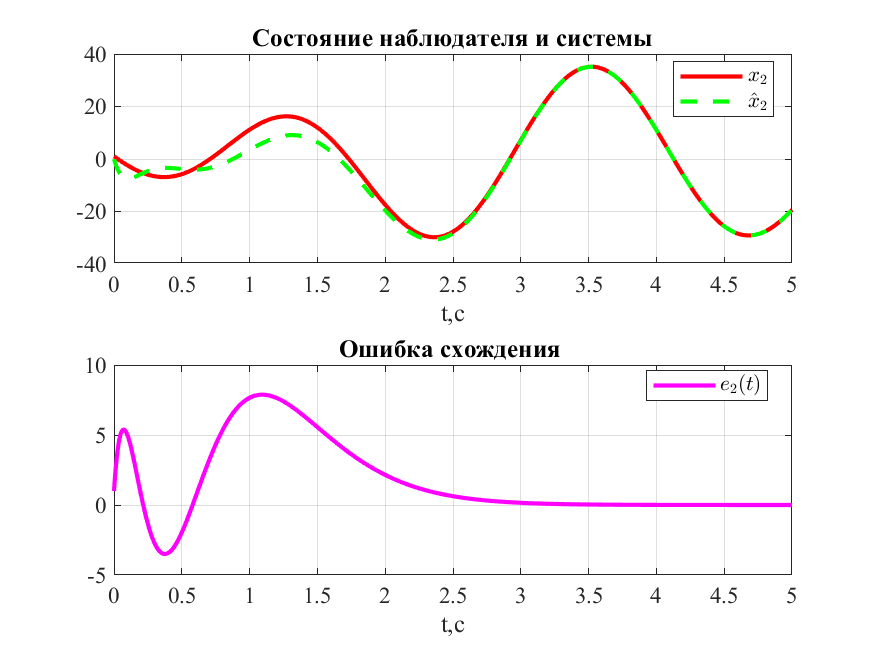
\includegraphics[width=0.8\textwidth]{obsv2.png}
  \caption{Состояние системы и наблюдатель }
\end{figure}
\begin{figure}[ht]
  \centering
  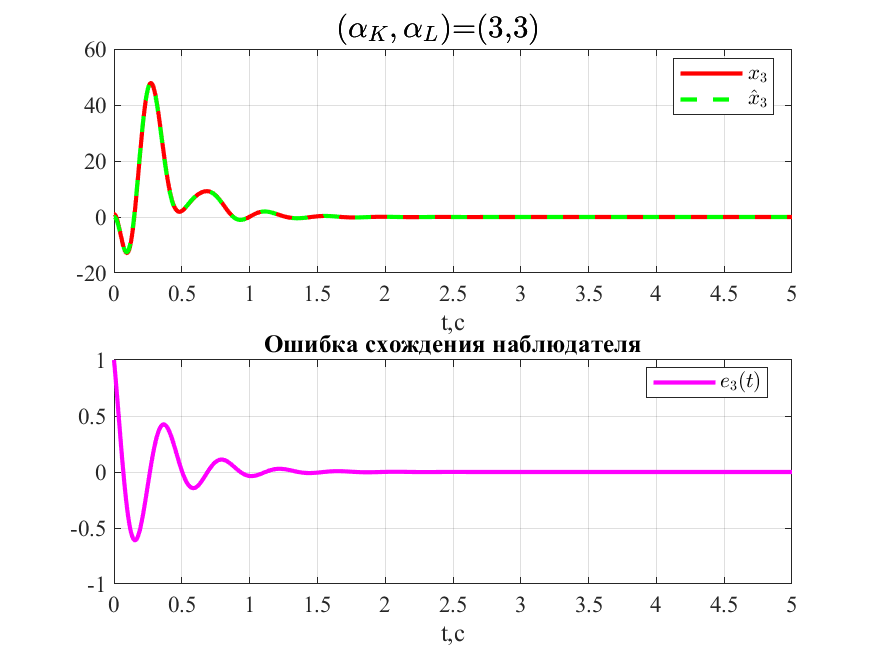
\includegraphics[width=0.8\textwidth]{obsv3.png}
  \caption{Состояние системы инаблюдатель}
\end{figure}
\newpage
\begin{figure}[ht]
  \centering
  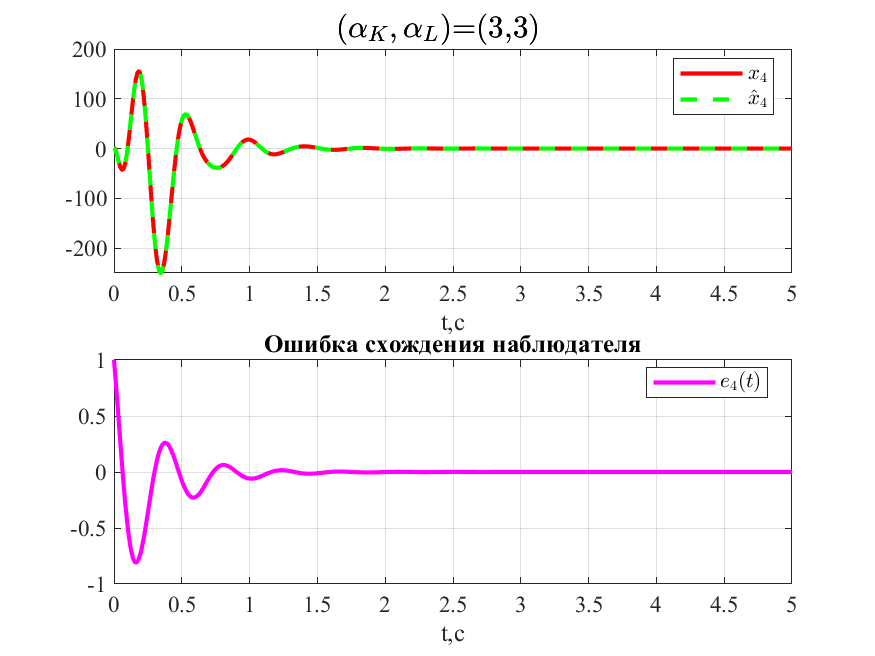
\includegraphics[width=0.8\textwidth]{obsv4.png}
  \caption{Состояние системы и наблюдатель}
\end{figure}
В дальнейшем формулы останутся теми же, поэтому исследования будут сжаты\dots

\newpage
$$
  \alpha_K = \alpha_L = 11
$$

Синтезируем регулятор при помощи \textbf{матричного уравнения Риккати}:
$$
\mu = 226, \tab K_2 = \begin{bmatrix}
                  103.28 & -134.43  &  66.44 &  32.68
                    \end{bmatrix}
$$
Регулятор даст следующий спектр, у нас сейчас $\alpha_K = 11$:
$$
  \sigma(A+BK_2) =\{ -11 \pm 23.74i, -11 \pm 3.47i \}
$$
Судя по спектру, регулятор синтезирован корректно. 

Теперь синтезируем наблюдателя при помощи \textbf{матричного уравнения Риккати}:
$$
\mu = 29, \tab L_2 = \begin{bmatrix}
                    32.43 &  -20.55 \\
                  -41.75 &    3.67 \\
                    -1.57 &   16.34 \\
                  -17.27 &   -6.93 
                    \end{bmatrix}
$$
Наблюдатель даст следующий спектр, у нас сейчас $\alpha_L = 11$:
$$
  \sigma(A+L_2 C) = \{-11 \pm 12.95i, -11 \pm 0.18i  \}
$$
Судя по спектру, наблюдатель синтезирован корректно, так как он не превышеает заданной $\alpha$.

\newpage
\begin{figure}[ht]
  \centering
  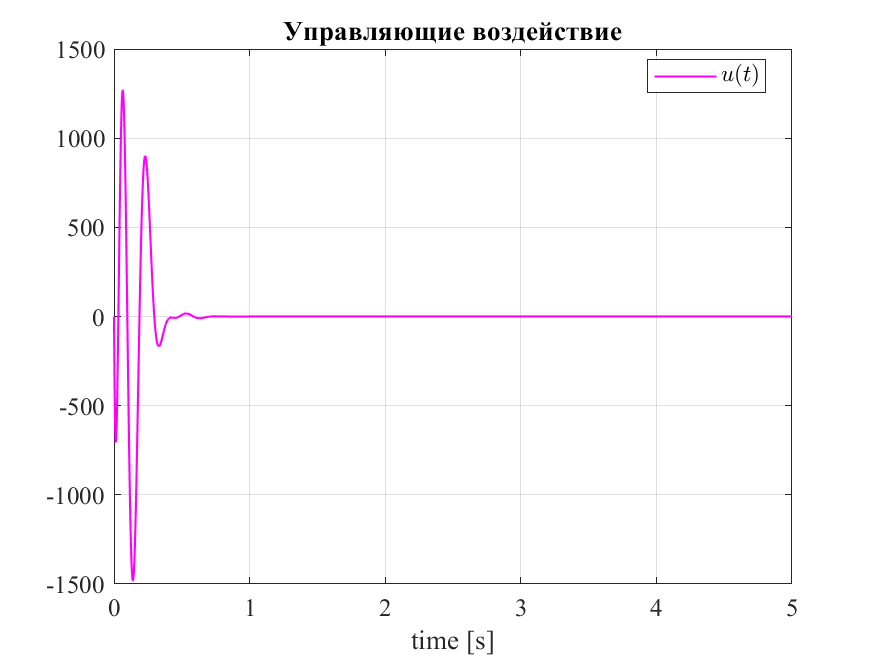
\includegraphics[width=0.8\textwidth]{obsv_u2.png}
  \caption{Сигнал управления}
\end{figure}
\begin{figure}[ht]
  \centering
  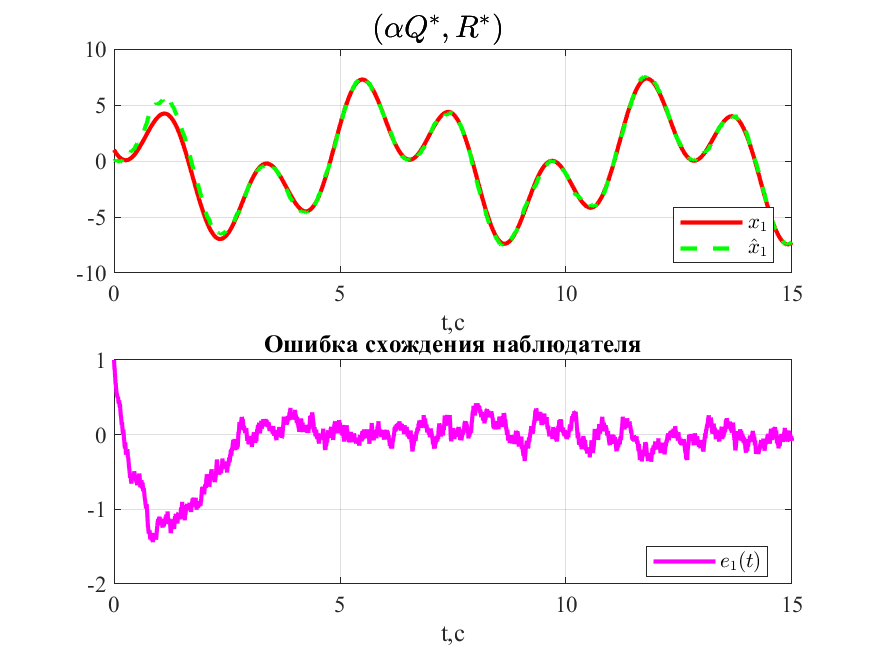
\includegraphics[width=0.8\textwidth]{obsv5.png}
  \caption{Состояние системы и наблюдатель}
\end{figure}
\newpage
\begin{figure}[ht]
  \centering
  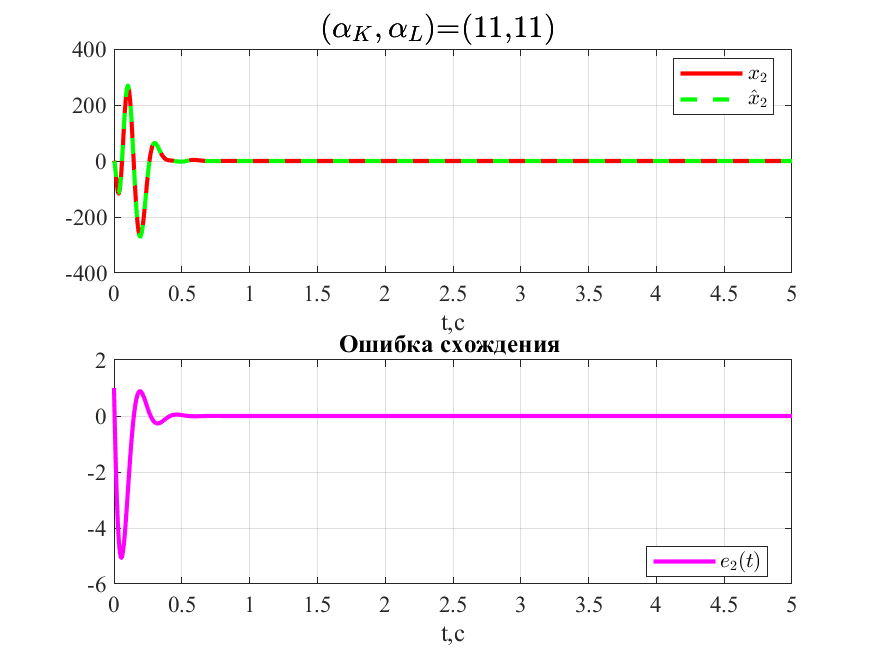
\includegraphics[width=0.8\textwidth]{obsv6.png}
  \caption{Состояние системы и наблюдатель}
\end{figure}
\begin{figure}[ht]
  \centering
  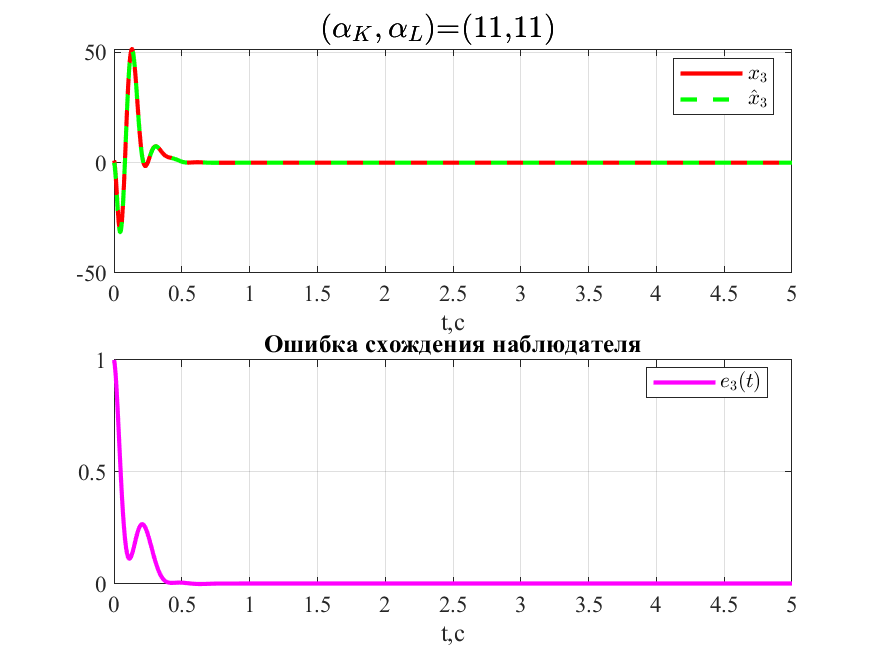
\includegraphics[width=0.8\textwidth]{obsv7.png}
  \caption{Состояние системы инаблюдатель}
\end{figure}
\newpage
\begin{figure}[ht]
  \centering
  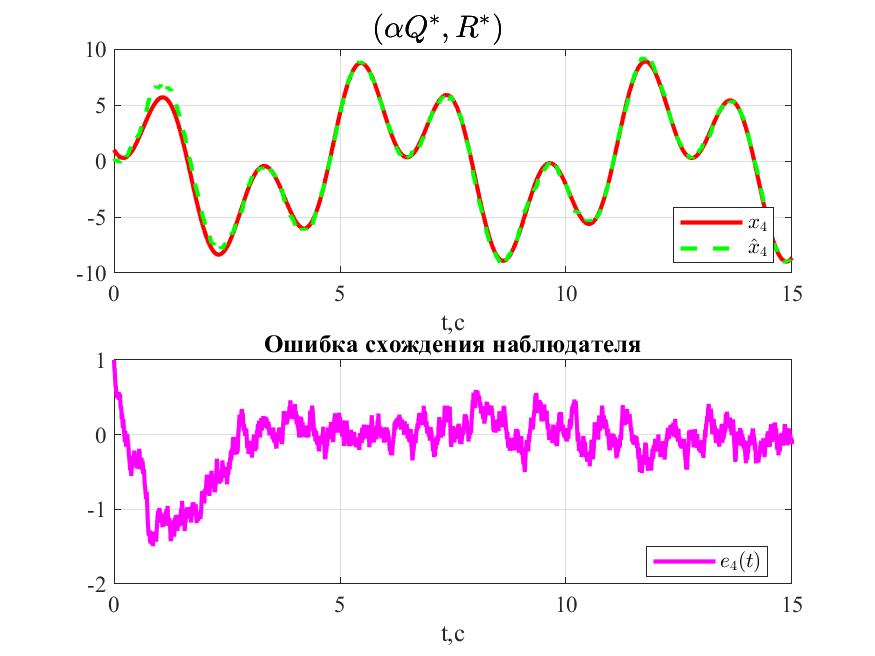
\includegraphics[width=0.8\textwidth]{obsv8.png}
  \caption{Состояние системы и наблюдатель}
\end{figure}
Можно заметить, что при увеличении параметра $\alpha: 3 \rightarrow 11$ мы значительно сократили перерегулирование и время переходного процесса, 
но взамен получили довольно резкое перерегулирование у контроллера во втором случае, посколько на него возлагалась более быстрая задача стабилизации сигнала. 
Примерно то же поведение можно наблюдать и у схождения наблюдателя к истинным компонентам вектора, всё-таки параметр $\alpha$ здесь равный и агрессивный.
\newpage
\subsection{Регулятор сильнее}
$$
  \alpha_K = 11, \tab \alpha_L = 3
$$
Синтезируем регулятор при помощи \textbf{матричного уравнения Риккати}:
$$
\mu = 226, \tab K_3 = \begin{bmatrix}
  225.14 & -304.37 & 175.49 & 84.6 \\
\end{bmatrix}
$$
Регулятор даст следующий спектр, у нас сейчас $\alpha_K = 11$:
$$
  \sigma(A+BK_3) =\{ -12.14 \pm 39i, -11 \pm 4i \}
$$
Судя по спектру, регулятор синтезирован корректно. 

Теперь синтезируем наблюдателя при помощи \textbf{матричного уравнения Риккати}:
$$
\mu = 29, \tab L_3 = \begin{bmatrix}
  20.47 & -17.44 \\
  -23.72 & 10.17 \\
  -4.74 & 6.02 \\
  -8.01 & -1.28 \\
\end{bmatrix}
$$
Наблюдатель даст следующий спектр, у нас сейчас $\alpha_L = 3$:
$$
  \sigma(A+L_3 C) = \{-3 \pm 14.68i, -3 , -8  \}
$$
Судя по спектру, наблюдатель синтезирован корректно, так как он не превышеает заданной $\alpha$.

\newpage
\begin{figure}[ht]
  \centering
  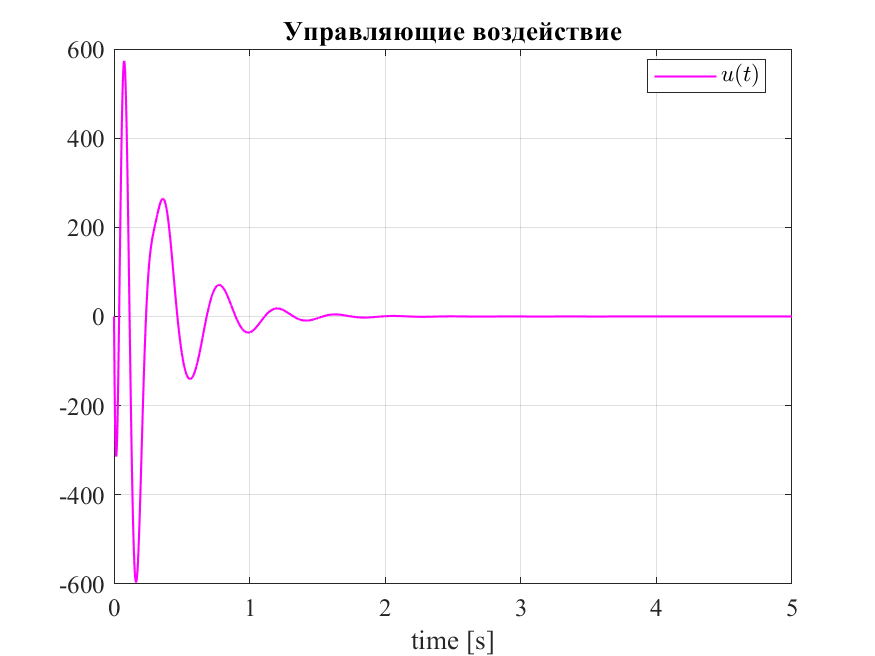
\includegraphics[width=0.8\textwidth]{obsv_u3.png}
  \caption{Сигнал управления}
\end{figure}
\begin{figure}[ht]
  \centering
  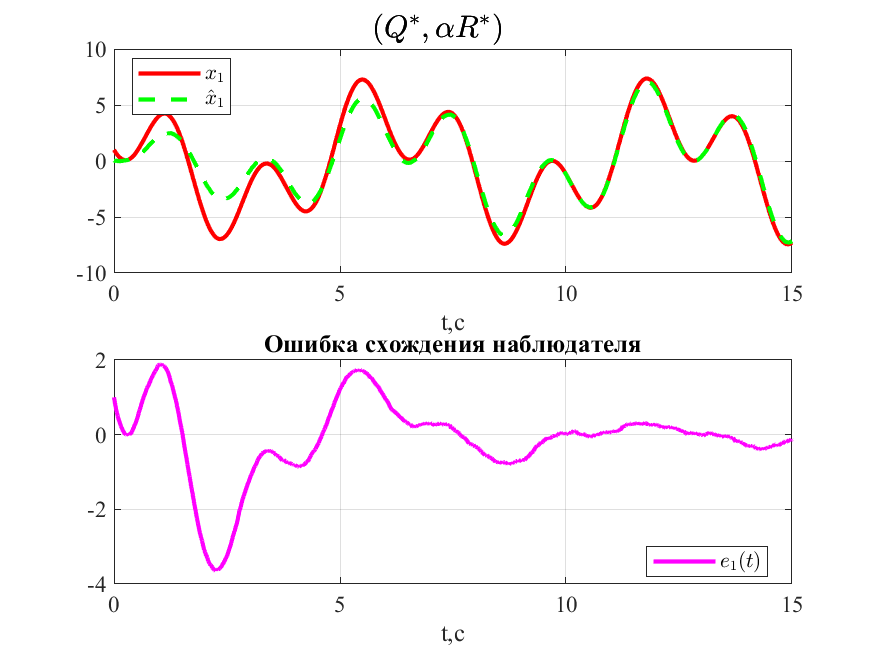
\includegraphics[width=0.8\textwidth]{obsv9.png}
  \caption{Состояние системы и наблюдатель}
\end{figure}
\newpage
\begin{figure}[ht]
  \centering
  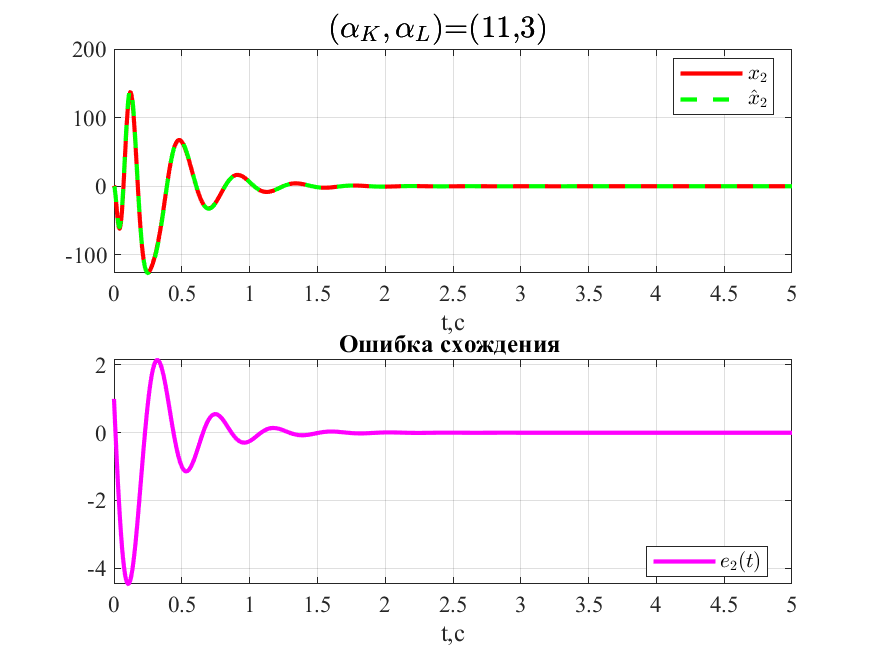
\includegraphics[width=0.8\textwidth]{obsv10.png}
  \caption{Состояние системы и наблюдатель}
\end{figure}
\begin{figure}[ht]
  \centering
  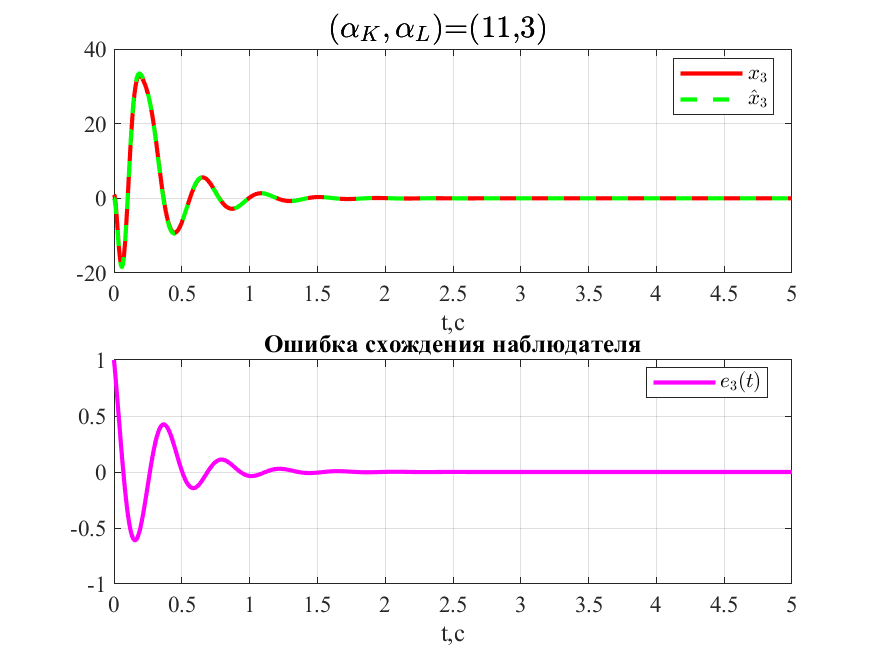
\includegraphics[width=0.8\textwidth]{obsv11.png}
  \caption{Состояние системы инаблюдатель}
\end{figure}
\begin{figure}[ht]
  \centering
  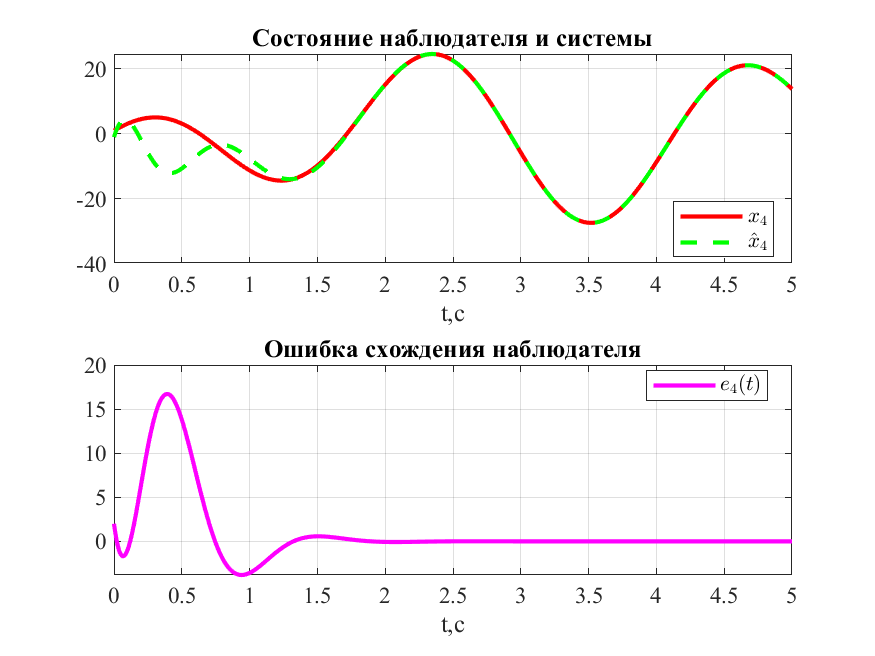
\includegraphics[width=0.8\textwidth]{obsv12.png}
  \caption{Состояние системы и наблюдатель}
\end{figure}

Сейчас можно заметить другую тенденцию - мы оставили регулятору агрессивное поведение, поэтому получили резкое перерегулирование, но время переходного процесса увеличилось по сравнению с прошлым набором $(\alpha_K, \alpha_L)=(11, 11)$, поэтому уже как минимум ясно, что выбор коррелирует. 
Сходимость наблюдателя осталась же примерно такой же, как и в случае $(\alpha_K, \alpha_L)=(3, 3)$, поэтому такой сменой приоритетов в коэффцициентах мы повлияли лишь на регулятор.

\newpage
\subsection{Наблюдатель сильнее}
$$
  \alpha_K = 3, \tab \alpha_L = 11
$$

Синтезируем регулятор при помощи \textbf{матричного уравнения Риккати}:
$$
\mu = 26, \tab K_4 = \begin{bmatrix}
  48.64 & -60.44 & 24.37 & 12.56 \\
\end{bmatrix}
$$
Регулятор даст следующий спектр, у нас сейчас $\alpha_K = 3$:
$$
  \sigma(A+BK_4) =\{ -4.8 \pm 23.74i, -4.8, -7.97 \}
$$
Судя по спектру, регулятор синтезирован корректно. 

Теперь синтезируем наблюдателя при помощи \textbf{матричного уравнения Риккати}:
$$
\mu = 29, \tab L_4 = \begin{bmatrix}
  50.52 & -35.89 \\
  -60.2 & 18.51 \\
  -1.94 & 14.8 \\
  -18.81 & -9.26 \\
\end{bmatrix}
$$
 Наблюдатель даст следующий спектр, у нас сейчас $\alpha_L = 11$:
$$
  \sigma(A+L_4 C) = \{-11 \pm 23.20i, -11 \pm 6.27i  \}
$$
Судя по спектру, наблюдатель синтезирован корректно, так как он не превышеает заданной $\alpha$.

\newpage
\begin{figure}[ht]
  \centering
  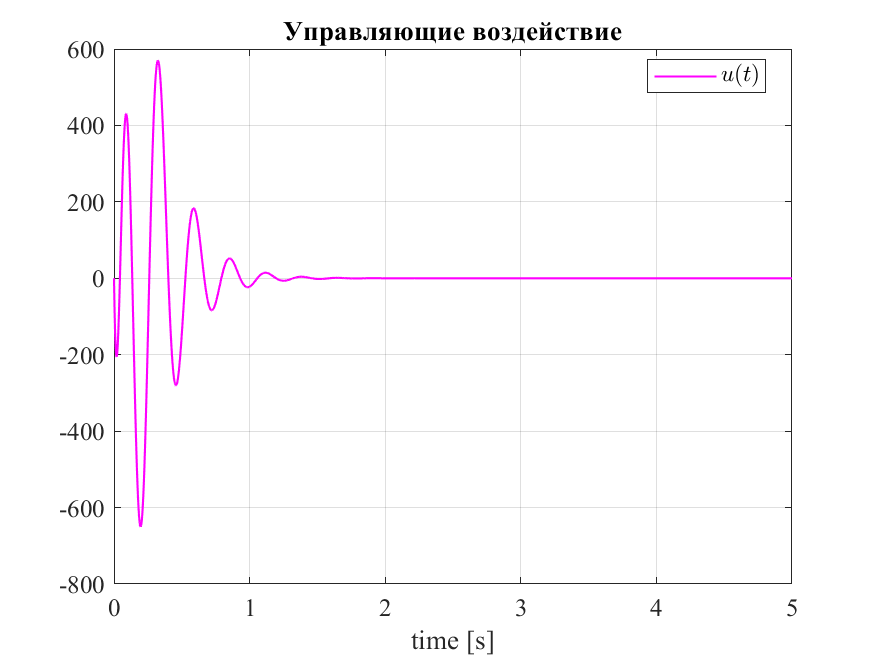
\includegraphics[width=0.8\textwidth]{obsv_u4.png}
  \caption{Сигнал управления}
\end{figure}
\begin{figure}[ht]
  \centering
  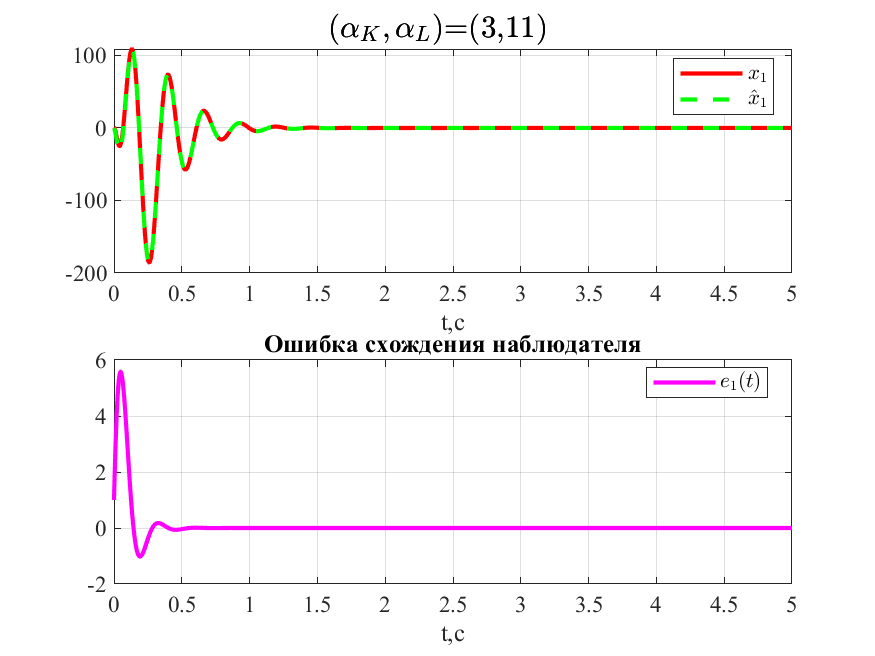
\includegraphics[width=0.8\textwidth]{obsv13.png}
  \caption{Состояние системы и наблюдатель}
\end{figure}
\newpage
\begin{figure}[ht]
  \centering
  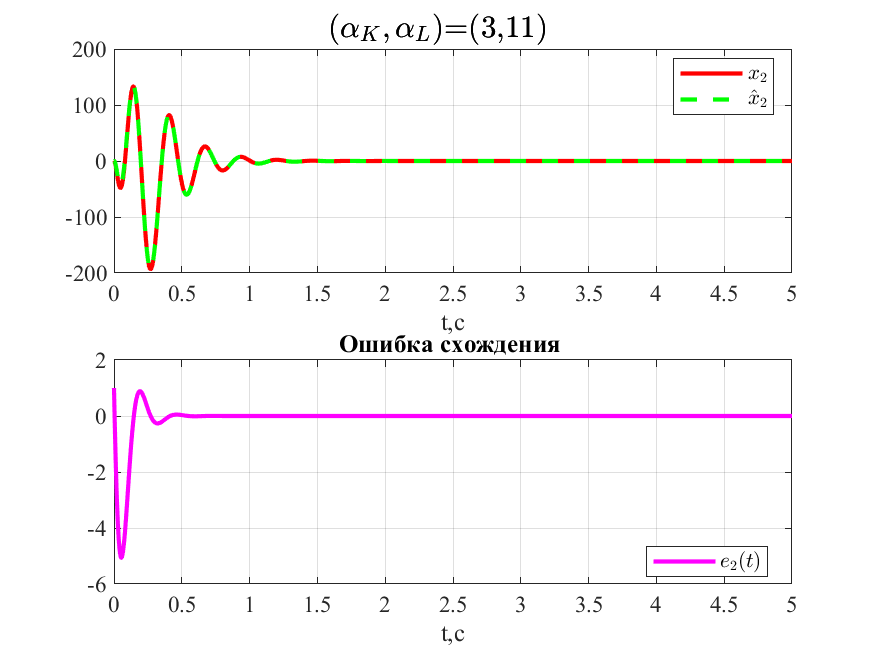
\includegraphics[width=0.8\textwidth]{obsv14.png}
  \caption{Состояние системы и наблюдатель}
\end{figure}
\begin{figure}[ht]
  \centering
  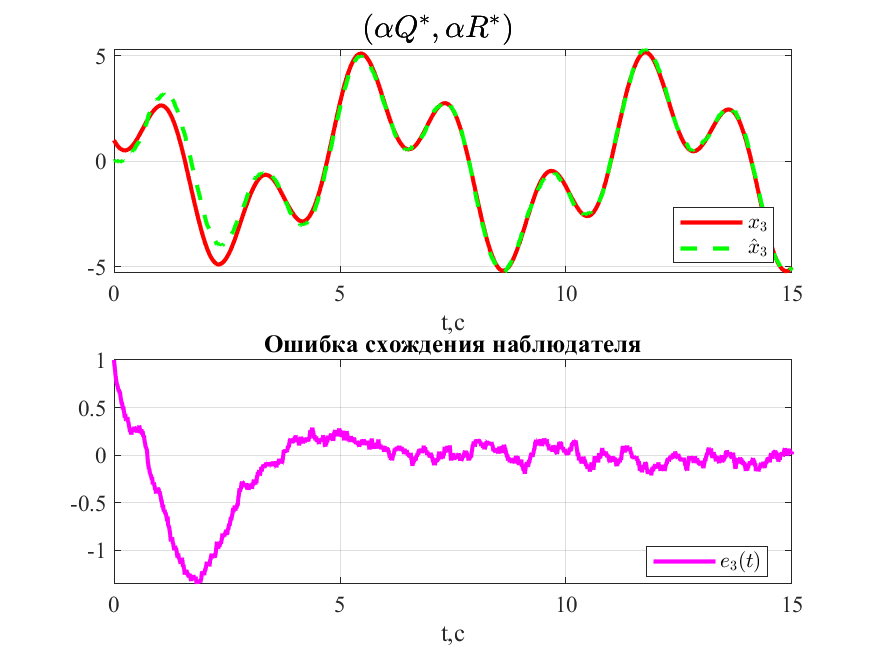
\includegraphics[width=0.8\textwidth]{obsv15.png}
  \caption{Состояние системы инаблюдатель}
\end{figure}
\newpage
\begin{figure}[ht]
  \centering
  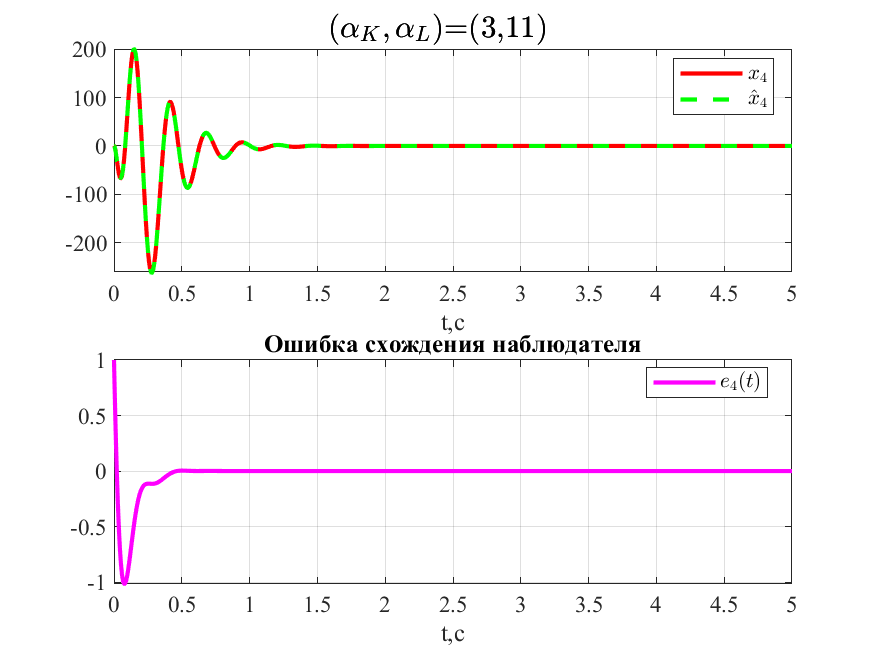
\includegraphics[width=0.8\textwidth]{obsv16.png}
  \caption{Состояние системы и наблюдатель}
\end{figure}

В данном случае тенденция перевернулась - мы дали наблюдателю агрессивное поведение, и его сходимасть стала аналогичной набору $(\alpha_K, \alpha_L)=(11, 11)$. Однако теперь корреляция сработала по-другому. 
Сигнал управления немного растянул своё `перерегулирование`, то есть время переходного процесса снова увеличилось.



\subsection{Вывод}
В этом задании мы работали с полностью наблюдаемой/управляемой системой, для неё мы синтезировали наблюдателя и регулятора с заданной степенью устойчивости, регулируемой выбором коэффициента $\alpha$.

Мы сравнили разные конфигурации выбора $\alpha$, которые показали нам, что выбор агрессивной политики у наблюдателя и регулятора (большие $\alpha$) показывают ожидаемые результаты - мы получаем быструю и качественную сходимость. 

При выборе же разных коэффцициентов $\alpha$, при выборе приоритета, то есть дать бОльшую сходимость регулятору или наблюдателю - мы видим их некоторую взаимосвязь. Она проявляет себя в том, что более сильная компонента ухудшает точностные свойства слабой.
\endinput 